\documentclass{article} % For LaTeX2e
% We will use NIPS submission format
\usepackage{nips13submit_e,times}
% for hyperlinks
\usepackage{hyperref}
\usepackage{url}
% For figures
\usepackage{graphicx} 
\usepackage{subfigure} 
% math packages
\usepackage{amsmath}
\usepackage{amsfonts}
\usepackage{amsopn}
\usepackage{ifthen}
\usepackage{natbib}

\title{Project-I by Group Sydney}

\author{
Diego Antognin and Jason Racine \\
EPFL \\
\texttt{diego.antognini@epfl.ch}, \texttt{jason.racine@epfl.ch} \\
}

% The \author macro works with any number of authors. There are two commands
% used to separate the names and addresses of multiple authors: \And and \AND.
%
% Using \And between authors leaves it to \LaTeX{} to determine where to break
% the lines. Using \AND forces a linebreak at that point. So, if \LaTeX{}
% puts 3 of 4 authors names on the first line, and the last on the second
% line, try using \AND instead of \And before the third author name.

\nipsfinalcopy 

\begin{document}

\maketitle

\begin{abstract}

\end{abstract}

\section{Regression}

\subsection{Data Description}

The train-data for regression consists of $N = 2800$ input ($\mathbf{X}$) and output ($\mathbf{y}$) data samples. Each input sample is a vector $\mathbf{x}_n$ with dimension $D = 76$. Out of these $76$ variables, $63$ are real, $3$ binary, $4$ categorical with 3 categories, $6$ are categorical with 4 categories.

We also have test-data of size $N=1200$ without their corresponding output. Our goal is to produce predictions for those data, as well as an approximation of the test-error.

\subsection{Data visualization and cleaning}

We first have plot the distribution of our features (plot not shown because too big for the $76$ features). As expected, they are not center and we should normalized them (each cluster will be normalized independently). The Figure \ref{fig:histogram} shows an histogram of the output ($\mathbf{y}$) and we can conclude our data  seem to be a combination of three Gaussian distributions. It will be used later in order to separate the data in three sets and apply different regression models on them. We can also observe that each cluster have different sizes : 1946, 576 and 278. Moreover, on the right, we can see some data points (there are $2$) which have a higher values than the others. We consider them as outliers and we will remove.

To separate the data, we have observed that the feature $2$ and $16$ could help us. Figure \ref{fig:feature2}. We can observe $11$ misclassified data (green points), which we will remove them in order to not corrupt our model.  So, this feature can allow us to find the first cluster. For the two others clusters, we need to oberve the feature $16$. Figure \ref{fig:feature16}. We can observe $14$ misclassified data (green points and one blue). They also will be consider as outliers and remove. We set the threshold in order to minimize the number of misclassified data samples. Those thresholds are $0.42$ for the feature $2$ and $1.17$ for the feature $16$.

We are also interested about the correlation between the input and output variables. We have observed the correlation for each cluster and conclude that for the first cluster, they are mainly in $[-0.1,0.1]$, except two features which are highly correlated. For the second and third cluster, also mainly in $[-0.1,0.1]$ but this time, there are more correlated features (~15). Moreover, the features seem not have correlation between them.

We use dummy encoding for the categorical variables (for a categorical variable of size $k$, we need $k-1$ features), which gives us a total of $93$ input variable.

We can note that the rank of our input matrix $\mathbf{X}$ is rank-deficient with a rank of 66 instead of 76, and is rank-deficient of 65 for each cluster.

\begin{figure}[!t]
\center
\subfigure[Histogram of $\mathbf{y}$. We can see three Gaussian distributions and also some outliers on the right.]{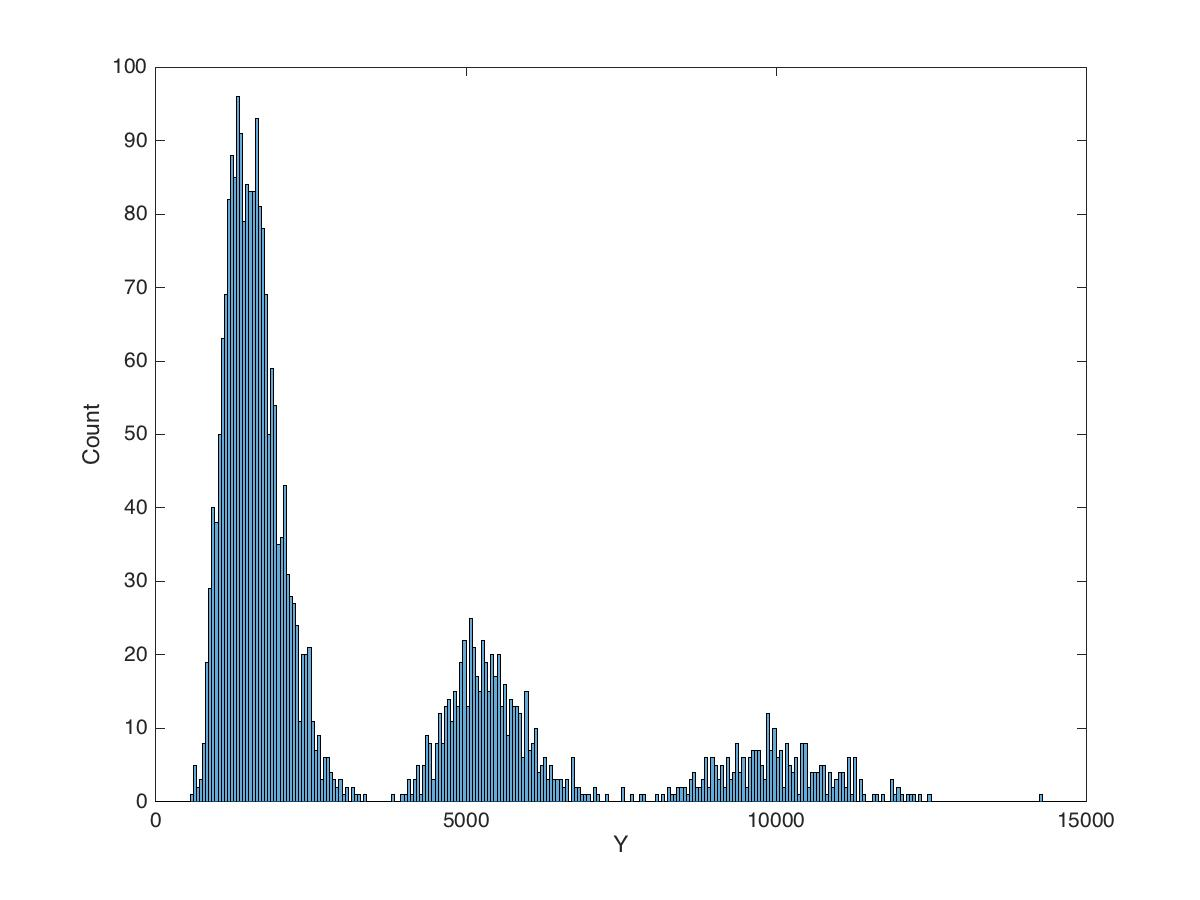
\includegraphics[width=2.5in]{figures/histogram.jpg} \label{fig:histogram}}
\hfill
\subfigure[Feature 2, because we have assumed that the data was generated from three Gaussian, this feature can help us to separate the data. Green data points are misclassified data. The separation is at $x=0.42$.]{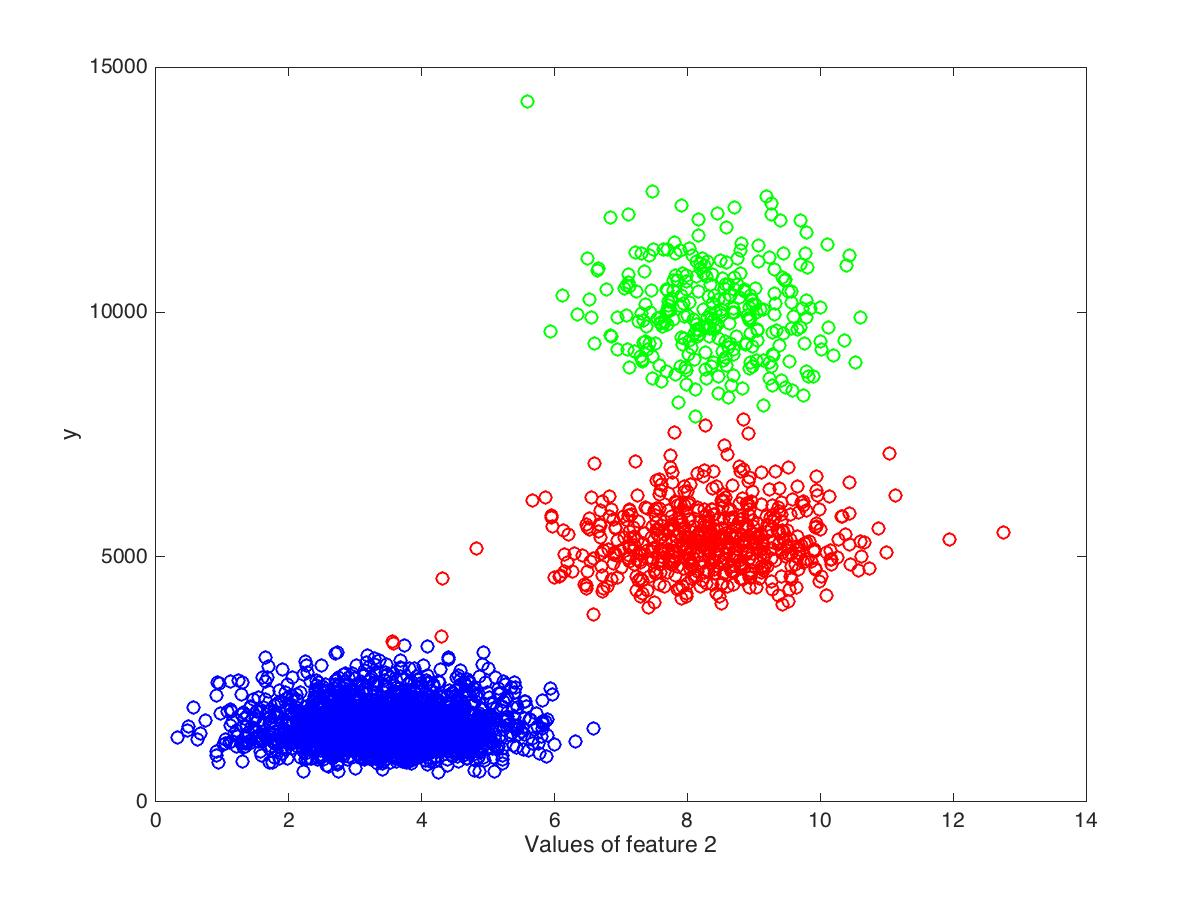
\includegraphics[width=2.5in]{figures/feature2.jpg}\label{fig:feature2}}
\hfill
\subfigure[Feature 16, because we have assumed that the data was generated from three Gaussian, this feature can help us to separate the data. Green data points are misclassified data. We can see see a blue data point which is misclassified, it will be an outlier. The separation is at $x=1.17$.]{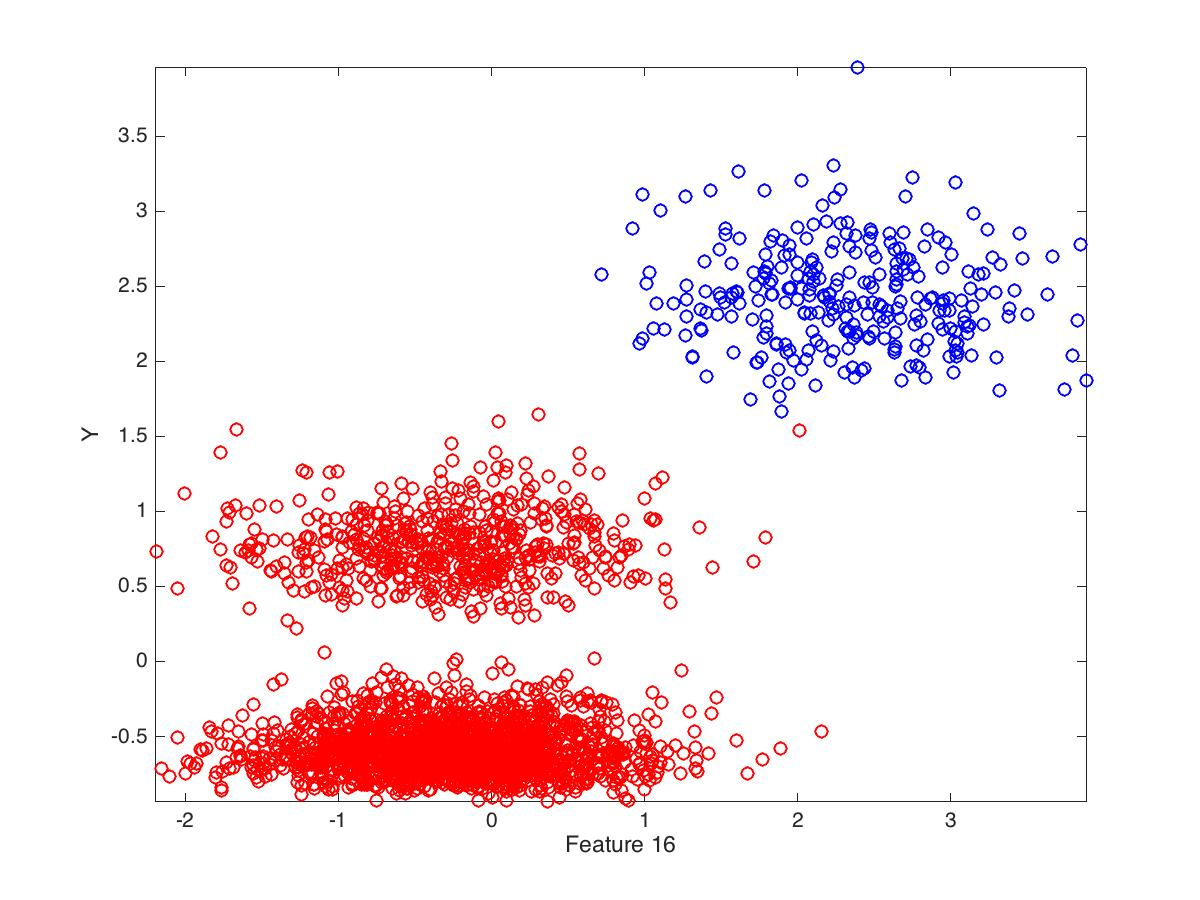
\includegraphics[width=2.5in]{figures/feature16.jpg}\label{fig:feature16}}
\hfill
\caption{}
\end{figure}

\subsection{Ridge Regression}

Since our matrix is ill-conditioned, using the least squares with normal equation wasn't suitable. Moreover, the results obtained were less good (not so much) compared to the ridge regression method, and so we will not report the results obtained with this method. The method using the least squares with gradient descent was appropriated, but compared to the ridge regression, it was a little bit less efficient and was also slower to tune correctly the learning step. This is the reason why we will not report the results using this method. Therefore, we have so used the ridge regression method, which is suitable because we should lift the eigenvalues, faster and a little bit more efficient than least squares using gradient descent. Only results obtained with this latter will be reported.

\subsubsection{Evaluation methods}

In order to evaluate our different models, we first have split our data ($\mathbf{X}$) in two sets of $80\%$ and $20\%$, for the training and the test sets. We learn with our models on the training set and use the test set in order to estimate the error using the \textit{Root Mean Square Error}. Moreover, we have also used k-cross validation (see next section for the values of k). We repeated the experiment $100$ times with different seed in order to split the data in a unique random way for each trial. Finally, we made varied the lambda from $10^{-5}$ to $10^{5}$ with $500$ values between.

\subsubsection{Model comparison}

The figure XXX represents the \textit{RMSE} for each models. The first model used in the constant one, which will allow us to compare improvements with others model. It simply returns the value of the mean of the outputs and doesn't depend on the inputs. Our second model consists of using also a constant model as in first, but this time separating the data in the three clusters identified during the exploratory data analysis. We can observed a big improvement, justifying our choice to split the data in clusters. 

The third model does a ridge regression on the overall data, in order to check that the separation of the data into clusters is better, even using only constant model per cluster. Hopefully, this is the case. The next model add the normalization on the input variables, another way to check if the separation of the data into cluster was a good things. Normalization is generally a good thing and often a necessity depending on the algorithms used (e.g. gradient descent ones). It improves only slightly but because normalization is a good practice, we keep it.

The fifth model consists of the separation of the data, using the normalization per cluster and finally does a ridge regression per cluster. With this manner, we can tune each cluster independently. We can see an important improvement because of the separation of the data. The next model adds the dummy encoding for the categorical variables. We can observe that it seems to be equivalent.

The seventh model is about using polynomial basis functions for each cluster. We have to be careful about the polynomial to avoid the case where $D > N$ (especially for the cluster two and three, because there are much smaller than the first one). This model doesn't use dummy encoding and so can add higher polynomial. The degrees of the polynomial for the clusters are $3,6$ and $3$. When we add higher degrees, we can directly observe overfitting because suddenly the training error decreases to a value near zero and the test errors grows exponentially, and so we know that our degrees are not to high. The eight model is similar to the seventh one, except that this time it uses dummy encoding and have lower degrees : $3,5$ and $2$, due to the number of input variables ($92$ vs $76$). We can see that these feature transformations significantly improve the prediction accuracy compared to others model.

\subsubsection{Feature transformations}

In hope to minimize the error, we tried different feature transformations. The first try was add polynomial of them self as $X = [X X^2 X^3 ...]$ for which each cluster has is own degree. We made varied the different degrees and also the lambdas in order to keep the lambda which minimize the test error.

We also thought about removing some uncorrelated features, we tried to remove the most uncorrelated then remove also the second one etc, but unfortunately we didn't get improvements. The reason is that maybe a feature may not be correlated directly with the input, however a combination of uncorrelated feature might be highly correlated.

\end{document}
